\xchapter{Proof of Concept}{} %sem preambulo
\label{chap:useExample}

\acresetall 

\section{Proposed Method}\label{sec:method}

For this project development, the agile Scrum method has been used. In Scrum, projects are divided into cycles called sprints, with frequent meetings where the team can inform what is being done and think of ways to improve the process quickly. Scrum proposes constant project monitoring. Often the team will be meeting, exchanging experiences, evaluating what has been done, and re-planning what will be done next.

During the requirements gathering, developers and other stakeholders sought to raise and prioritize the needs of future software users (referred to as requirements). After the requirements gathering, in the requirements specification stage, developers made a detailed study of data collected in the previous activity, from where models were built to represent the software system being developed.

At the architectural design stage of the system, two basic activities were performed: architectural design (or high-level design) and detailed design (or low-level design). Some aspects were considered at this stage of system design, such as system architecture, the platform used, Database Manager System (DBMS) used, and graphical interface standard.

In the application development period, the backend and frontend components were created from the computational description of the design phase. Pre-existing software tools and class libraries were used to streamline activity. These tools and libraries were defined during the architectural design and were referenced in \cref{sec:WebAppFrondEnd,sec:WebAppBackEnd}.

For system validation, two main requirements were evaluated: the components and the behavior of who will use the application. For the first point, functional, integration, and security tests will be performed. For the second, this proof of concept was applied.

Appendix \ref{app:projectManagement} presents the activities for project management, the user stories, and non-functional requirements. 


\section{Use Example}\label{sec:workflow}

To accomplish this usage example, one Coffee supply chain will be defined and configured accordingly. The supply chain of coffee beans is a lengthy process that involves growing the beans, harvesting, hulling, drying, packing, bulking, blending, and finally roasting. In between this process, the beans go through international transporters, export sellers, and retailers like grocery stores, cafes, and specialty shops. A coffee tree can take four to seven years before it yields its first crop of beans. The harvesting process is a very labor-intensive exercise. Parts of the cherry must be removed to access the beans and need to be laid out to dry. Once the beans are dried, they are packaged into large sacks and passed onto the exporters. They are distributed to big companies in the coffee business who take these beans and put them in industrial roasting and distribution centers. The inventory stock from the roasting and distributing centers must be passed forward to retailers. Through a web of transport, these coffee beans are delivered to thousands of roasters, cafes, restaurants, grocery stores, and large chain retailers, where they finally will come to the final users who will taste its flavor. 

For this scenario, five steps will be taken: Extraction is the step where the coffee is growing and picking. Processing is when the beans are dry, roasting, grinding, and packaging. Distribution is when the packages are shipping. Retail is about selling the product, and the final step is the final user consumption.

Five fictitious business enterprises and a final customer are named as follows: Tasty Coffee Farm, situated in Brazil, is an extractor responsible for all the information regarding the extraction step in the supply chain. Café Brazilium is the manufacturer and is responsible for the processing step. There will be two distribution companies. The first is Edgard Cargo which is the Distributor company and is in charge of distribution details. This company will send the coffee produced in Brazil to the United States. The second is O'Neil DistInc, a competitor of the first one. Marques BigSales is a United States situated Delicatessen store and is at the helm of selling details. Allan Manoel Jr. is a customer who wants to experiment with Brazilian coffee for the first time. Being very curious, the customer would like to know the provenance and the information about the coffee he drinks and where the coffee has passed.

As actors, each company above will have one user configured in the platform:  

\begin{itemize}
\item Extractor: James Johnson.
\item Manufacturer: Donald Jackson.
\item Distribution: Elizabeth Taylor.
\item Distribution: Charlotte O'Neil.
\item Retailer: BigSales.
\item Customer: Allan Manoel Jr.
\end{itemize}

The first step when creating a new Supply Chain  is to create and configure the asset. The admin user makes this action. By going through the setup wizard, first, the asset's info is requested:

\begin{figure}[H]
\begin{center}
  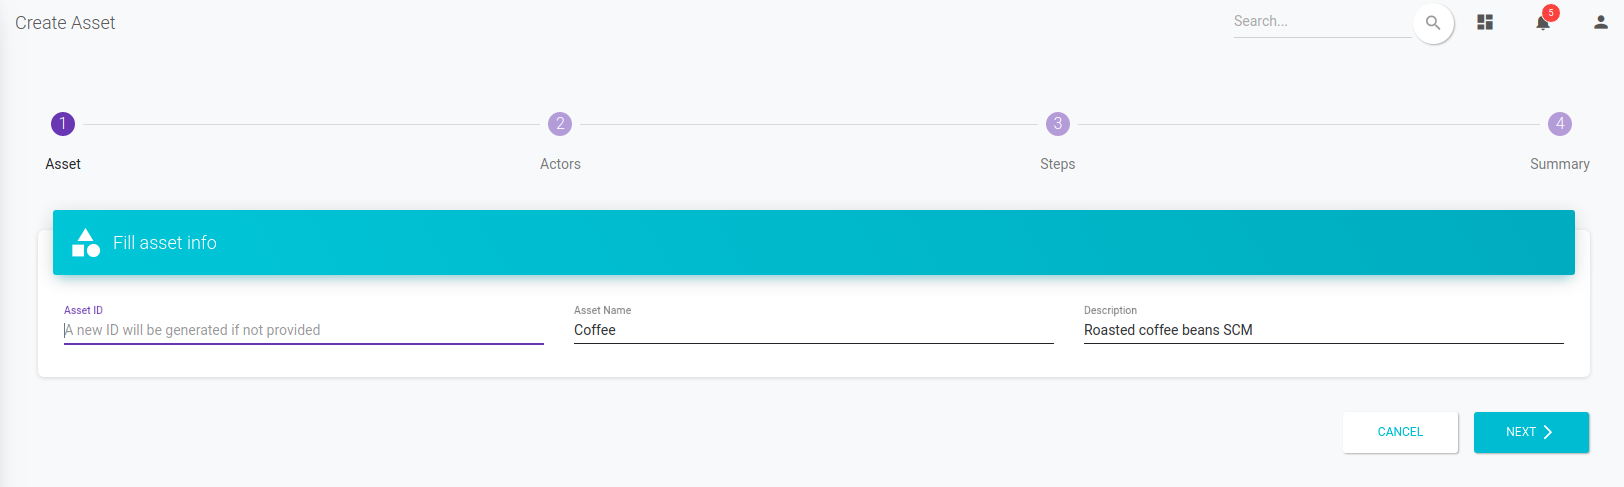
\includegraphics[scale=0.27]{images/use_example/01_create_asset_1.png}
\caption{Fill in asset info.}
\label{fig:create_asset_1}
\end{center}
\end{figure}

Then the admin will add actors to the SCM, informing its types. Actors can be added, updated, or deleted later on the actors' list page.

\begin{figure}[H]
\begin{center}
  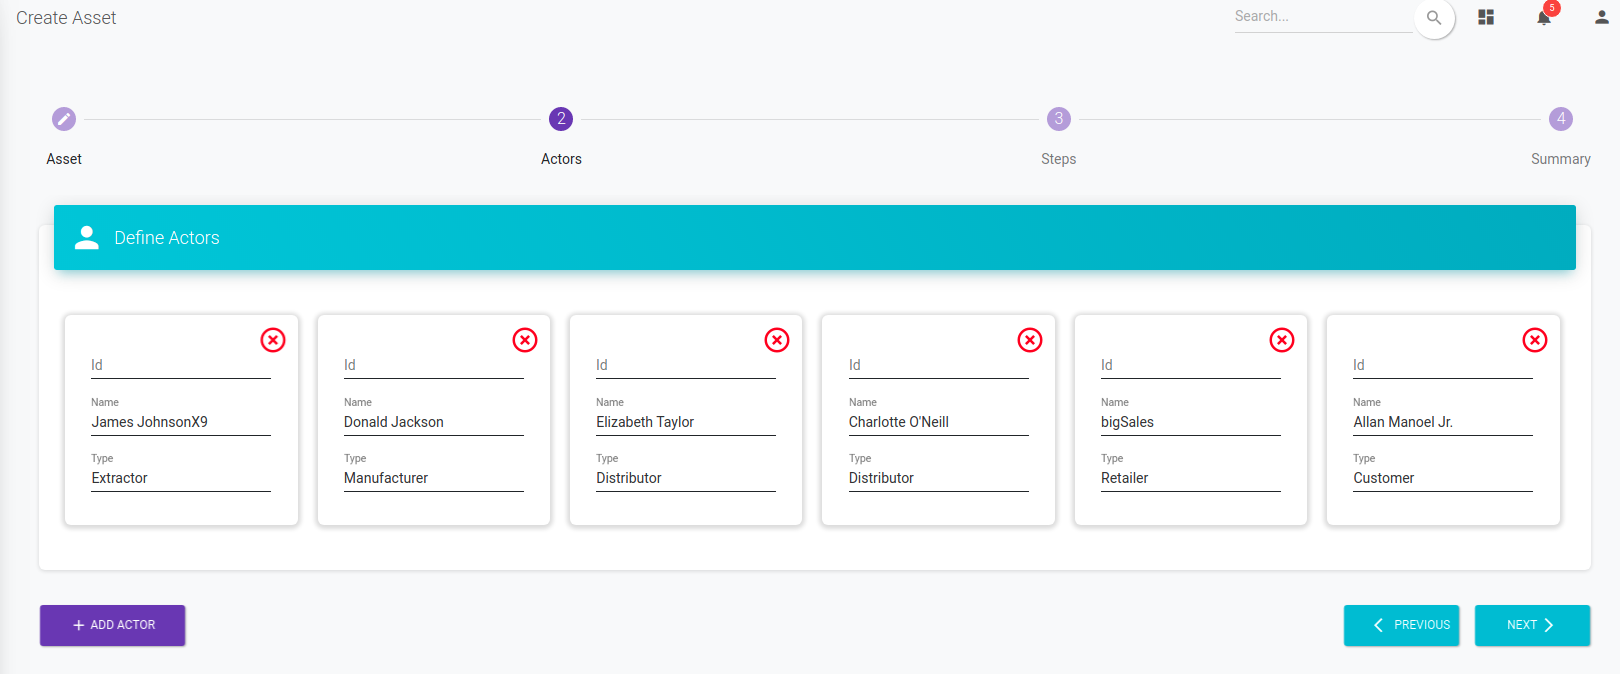
\includegraphics[scale=0.27]{images/use_example/02_create_asset_2.png}
\caption{Adding actors.}
\label{fig:create_asset_2}
\end{center}
\end{figure}


The next phase in the wizard is to define the Supply chain steps, specifying the order and binding it to the previous created actors' types:

\begin{figure}[H]
\begin{center}
  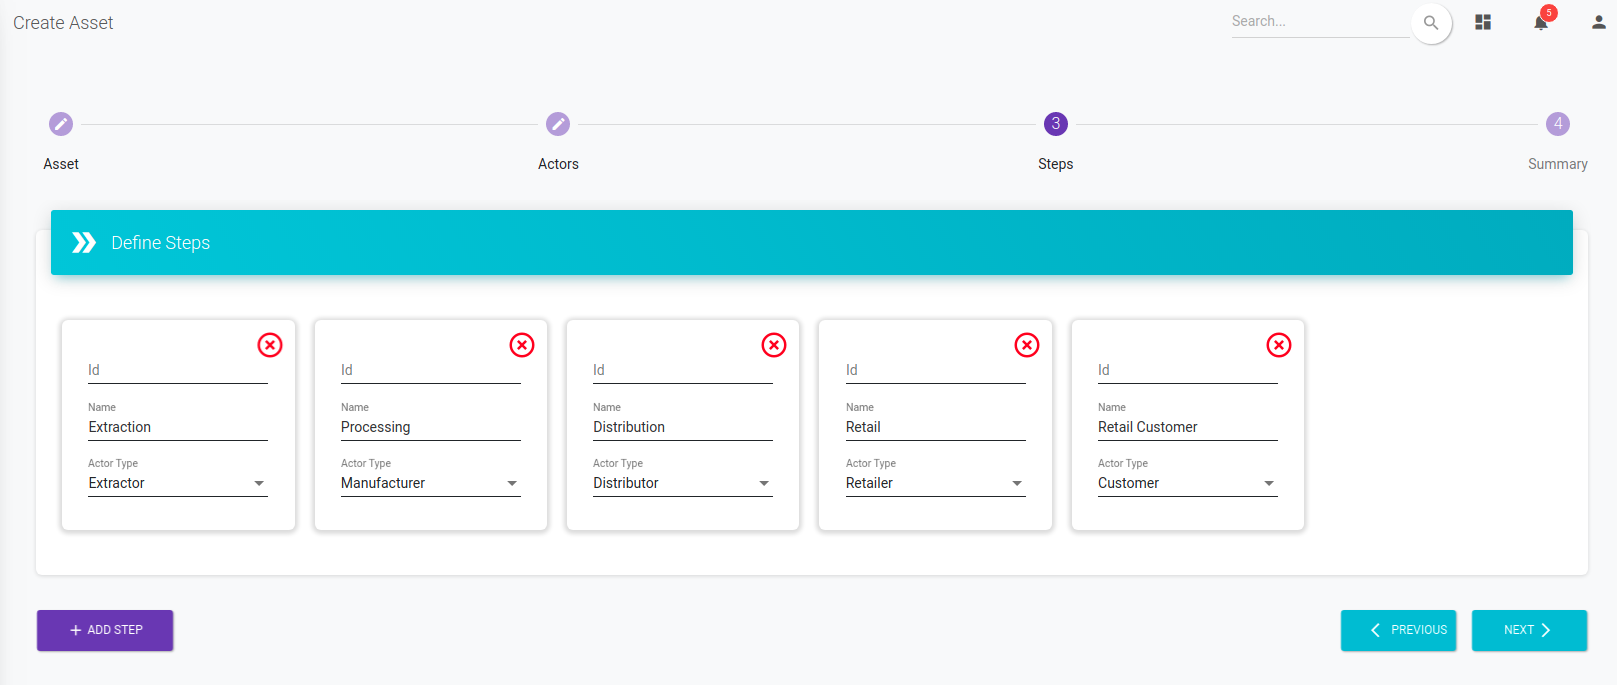
\includegraphics[scale=0.27]{images/use_example/03_create_asset_3.png}
\caption{Defining steps.}
\label{fig:create_asset_3}
\end{center}
\end{figure}

The final step, before submitting the form, is to review all the information previously added in the review asset details page, under the wizard:
\begin{figure}[H]
\begin{center}
  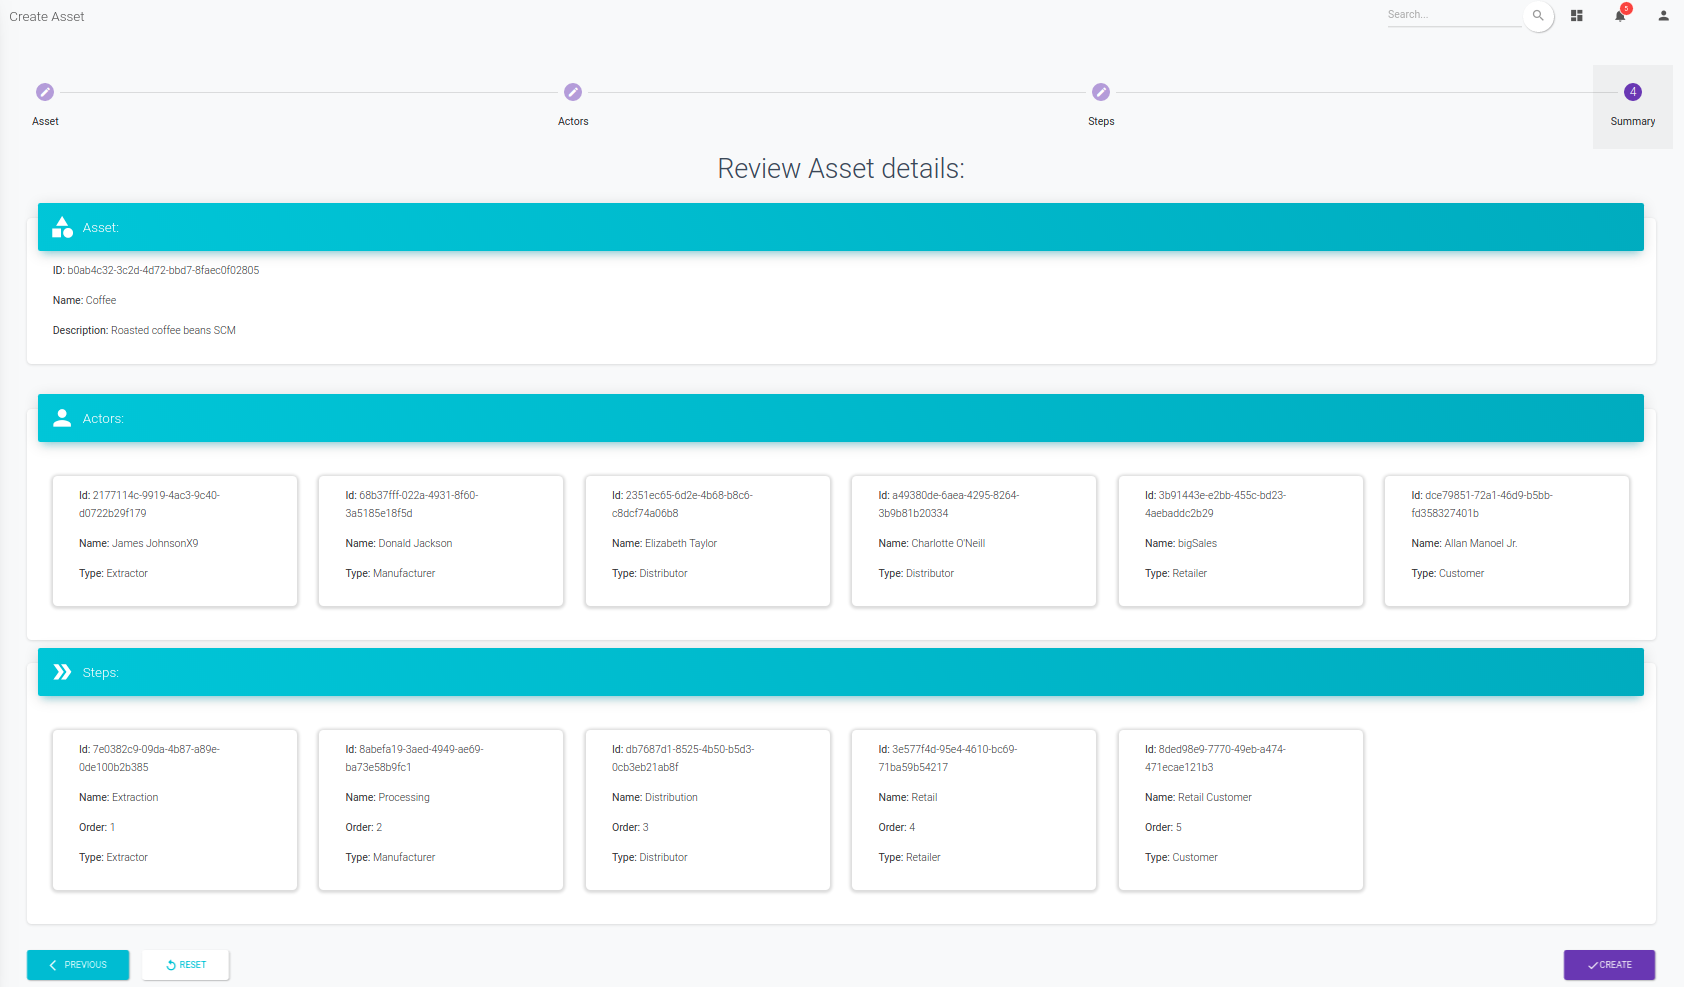
\includegraphics[scale=0.265]{images/use_example/04_create_asset_4.png}
\caption{Review asset details before submitting.}
\label{fig:create_asset_4}
\end{center}
\end{figure}


Once created, the asset can be seen in the assets list, where the admin can perform crud operations by the actions items. When clicking in the asset details, the current user is redirected to the asset details page, where the main information about asset items.
%, actors and steps can be seen. The card header contains a tab menu to provide navigation through these entities. 



% \begin{figure}[H]
% \begin{center}
%   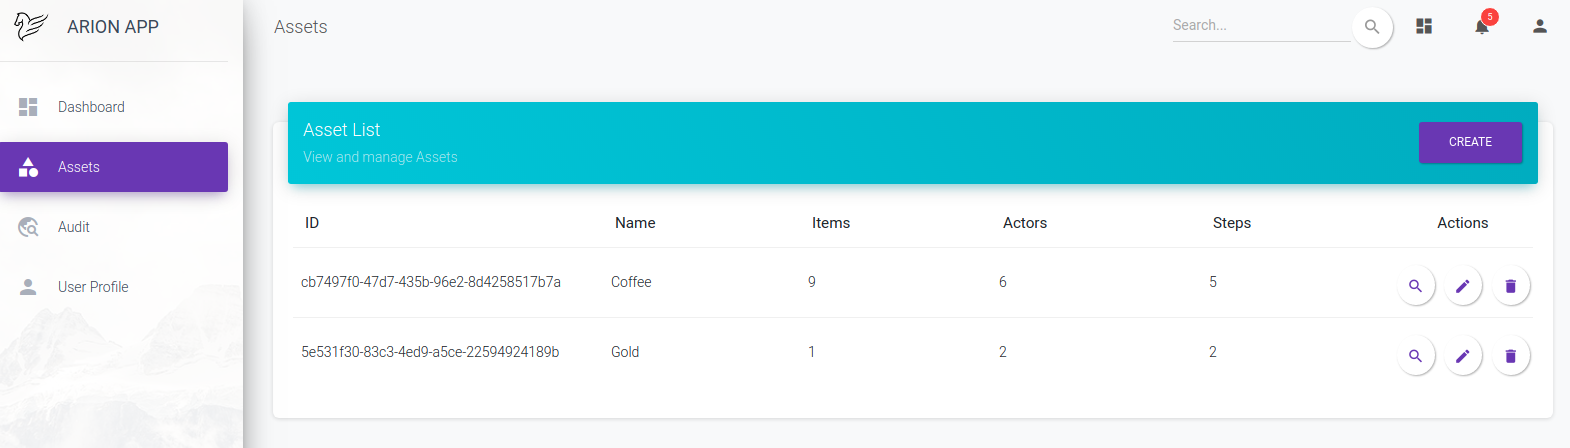
\includegraphics[scale=0.28]{images/use_example/05_asset_list.png}
% \caption{Asset list and action buttons.}
% \label{fig:asset_list}
% \end{center}
% \end{figure}



\begin{figure}[H]
\setlength{\belowcaptionskip}{-10pt}
\begin{center}
  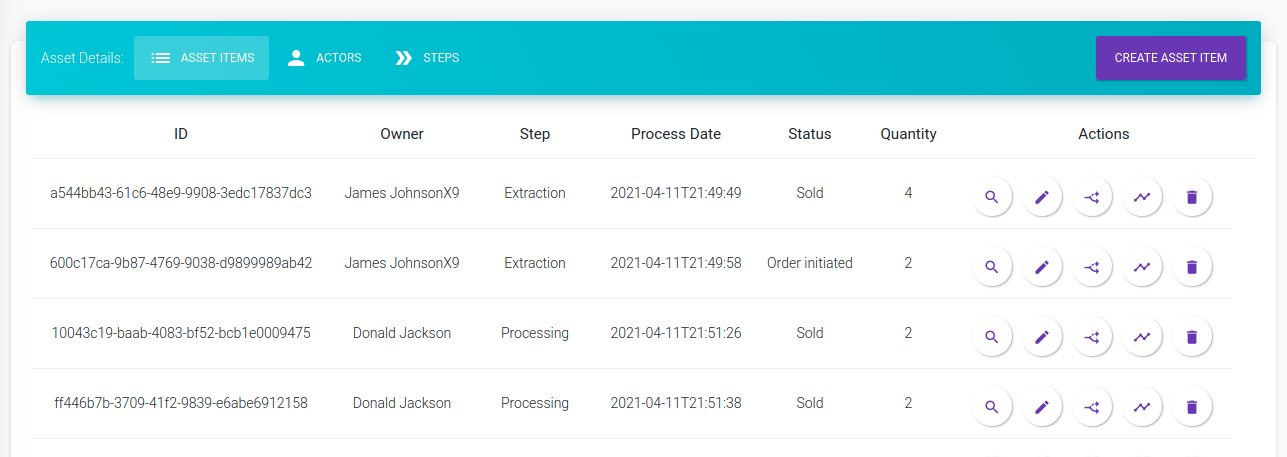
\includegraphics[scale=0.35]{images/use_example/06_asset_Item_list.png}
\caption{Asset Items list.}
\label{fig:asset_item_list}
\end{center}
\end{figure}

\begin{figure}[H]
\begin{center}
  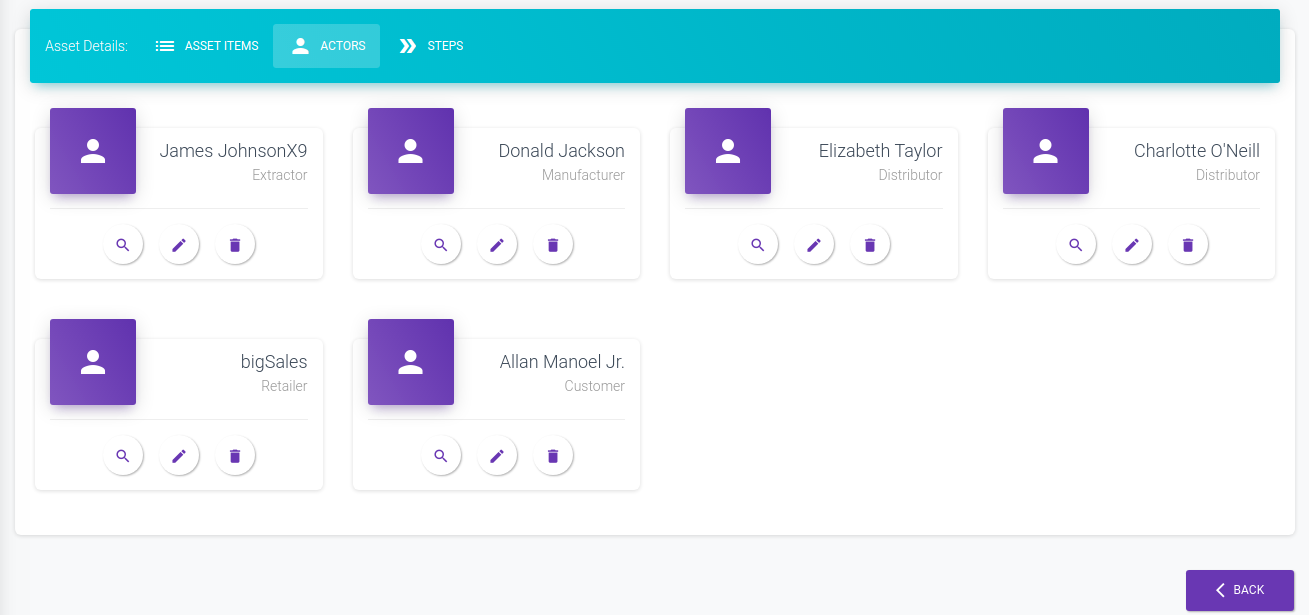
\includegraphics[scale=0.34]{images/use_example/07_actor_list.png}
\caption{Actors list.}
\label{fig:actor_list}
\end{center}
\end{figure}

\begin{figure}[H]
\begin{center}
  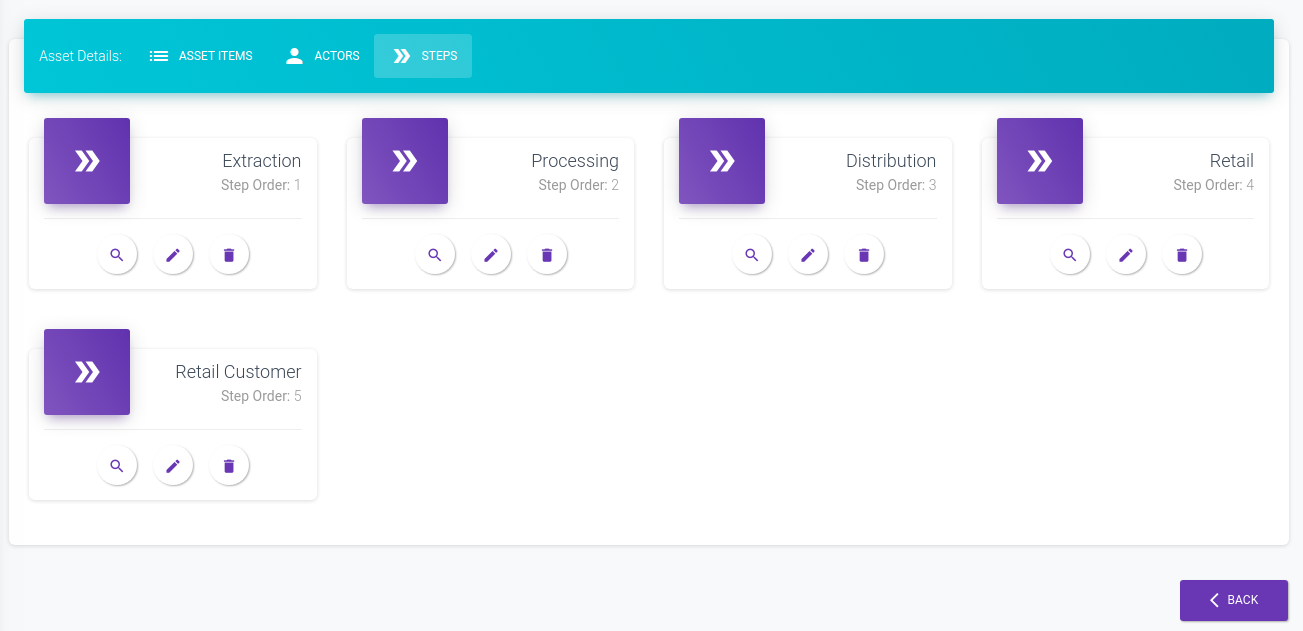
\includegraphics[scale=0.32]{images/use_example/08_steps_list.png}
\caption{Steps list.}
\label{fig:step_list}
\end{center}
\end{figure}

As an admin, there are also button actions to perform crud operations. Beyond Admins, actors responsible for the first step are allowed to create an asset item. This action will redirect the user to the create asset item form shown below. In the use case, a coffee crop was harvested by the extraction company. Information about this step is added at this point. 

\begin{figure}[H]
\begin{center}
  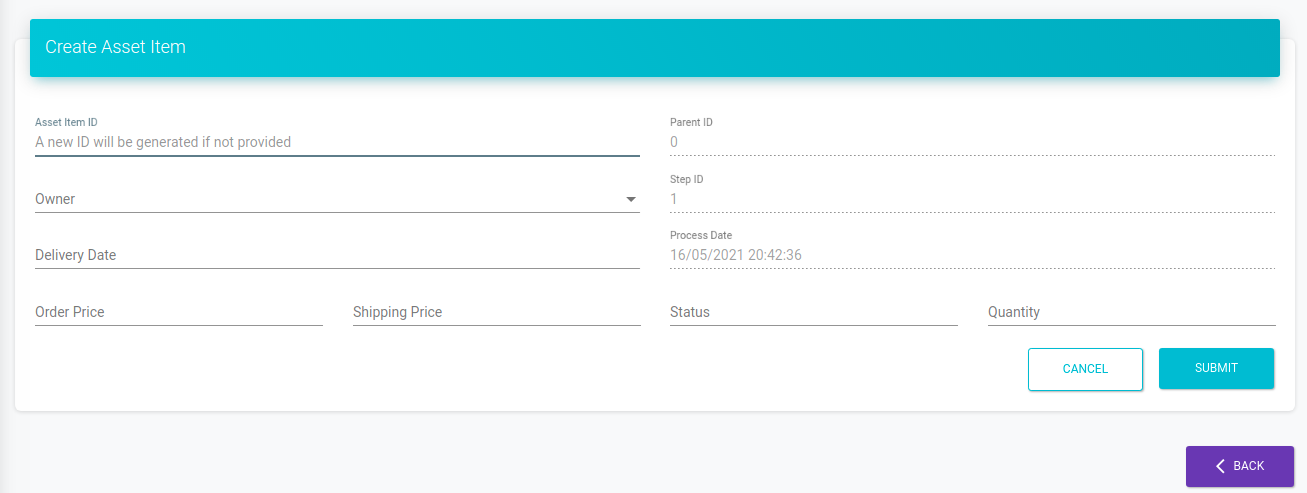
\includegraphics[scale=0.3]{images/use_example/09_create_asset_Item.png}
\caption{Create asset item form.}
\label{fig:create_asset_item}
\end{center}
\end{figure}


Beyond the crud actions in the asset items list, there are also two new actions: move asset item and track asset item. The first one shows a form where the user can move an asset through the SCM steps. The user can only move this asset item to the next or the previous step in the supply chain. Move an item back to the previous step is a feature that can be used when a customer needs to return the product to whoever sold it, for example, when a product comes defective, or the customer wants to exchange it. 

To the use case, the companies are using this feature to move towards the products. First, the Manufacturer company bought two lots from the same coffee crop of the extraction company. The manufacturer sold them into three lots after processing the products. The first and the second one were sent to the first distributor company and the third to the second distributor. The first distributor delivered the first lot to the retail company, and from this lot, a cup of coffee was sold to the final customer. All these actions were made from the moving asset item form below:

\begin{figure}[H]
\begin{center}
  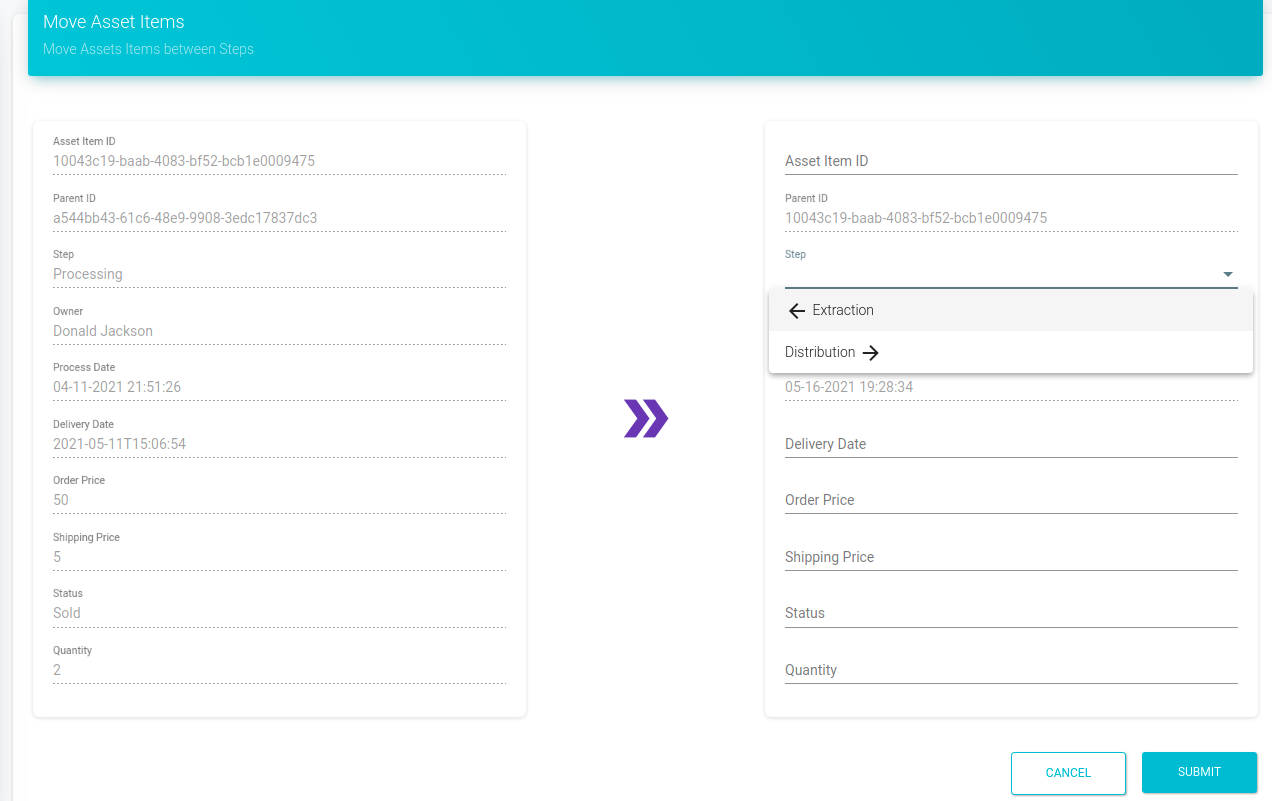
\includegraphics[scale=0.32]{images/use_example/091_move_asset_Item.png}
\caption{Move asset item form.}
\label{fig:move_asset_item}
\end{center}
\end{figure}

Track asset item displays the tracked info about the chosen asset item. It shows the children's tree of the selected element and its ancestors. Figure~\ref{fig:track_asset_item} shows the current status of the scenario described above by viewing the first asset item selected (the extracted coffee crop).

When clicking on a node in the chart, the information about the selected node is displayed under the diagram. Using this feature, the final user can track and see back that its cup of coffee has been passed. This information would be essential if a problem occurred. All the companies involved in this process could also track this information to understand better what happened, identify the possible step where a problem arose, and provide input for decision making.

\begin{figure}[H]
\begin{center}
  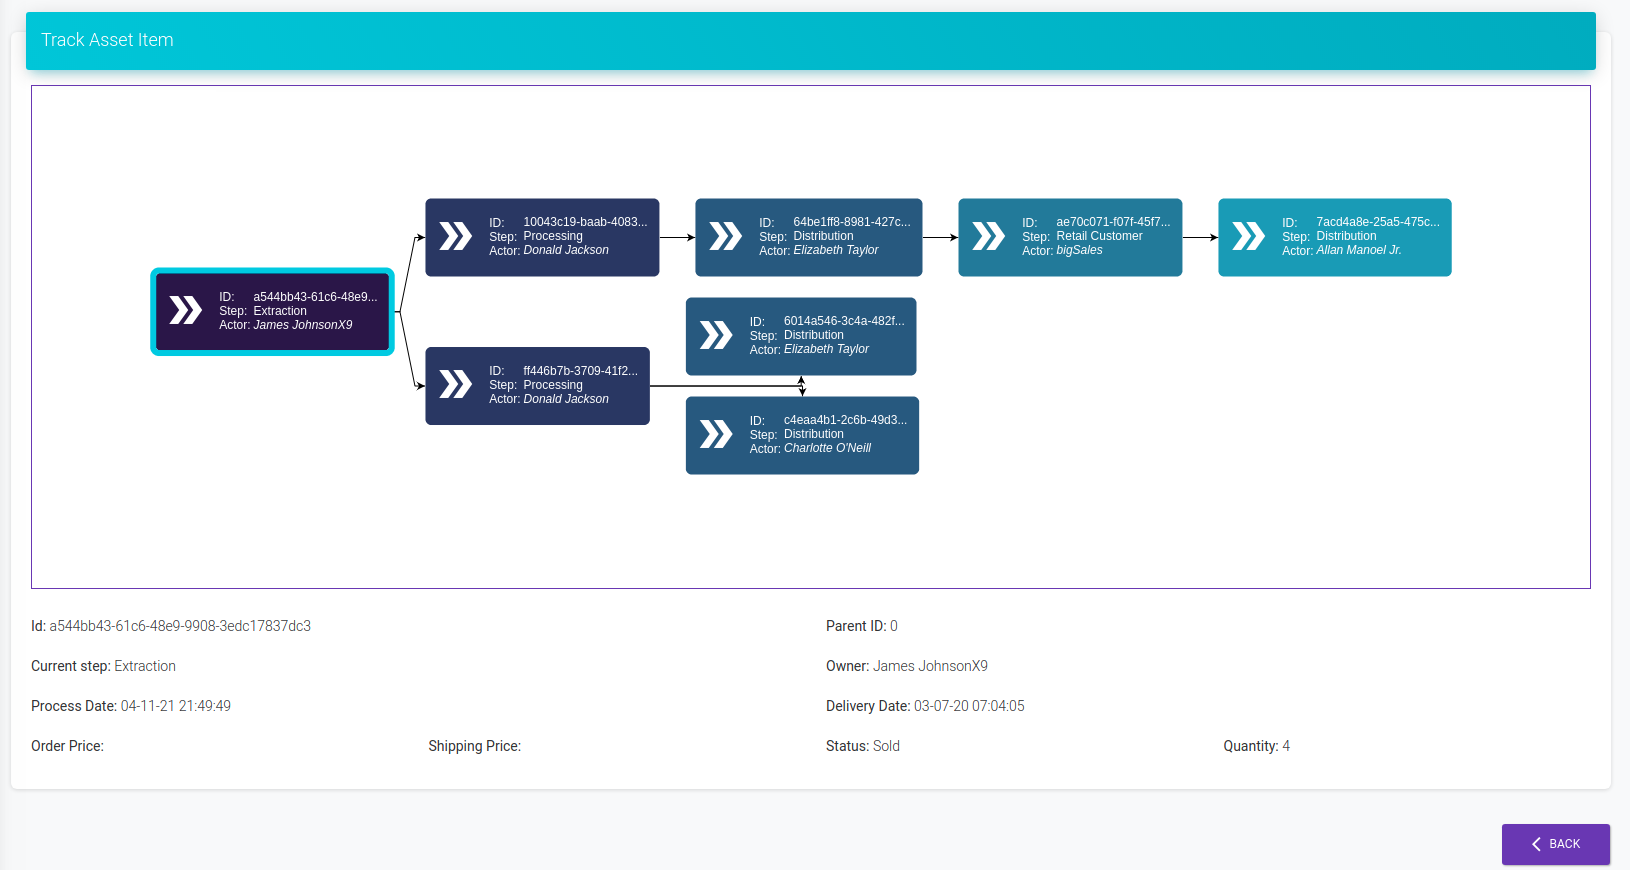
\includegraphics[scale=0.275]{images/use_example/092_track_asset_Item.png}
\caption{Track an asset item forward.}
\label{fig:track_asset_item}
\end{center}
\end{figure}


\begin{figure}[H]
\begin{center}
  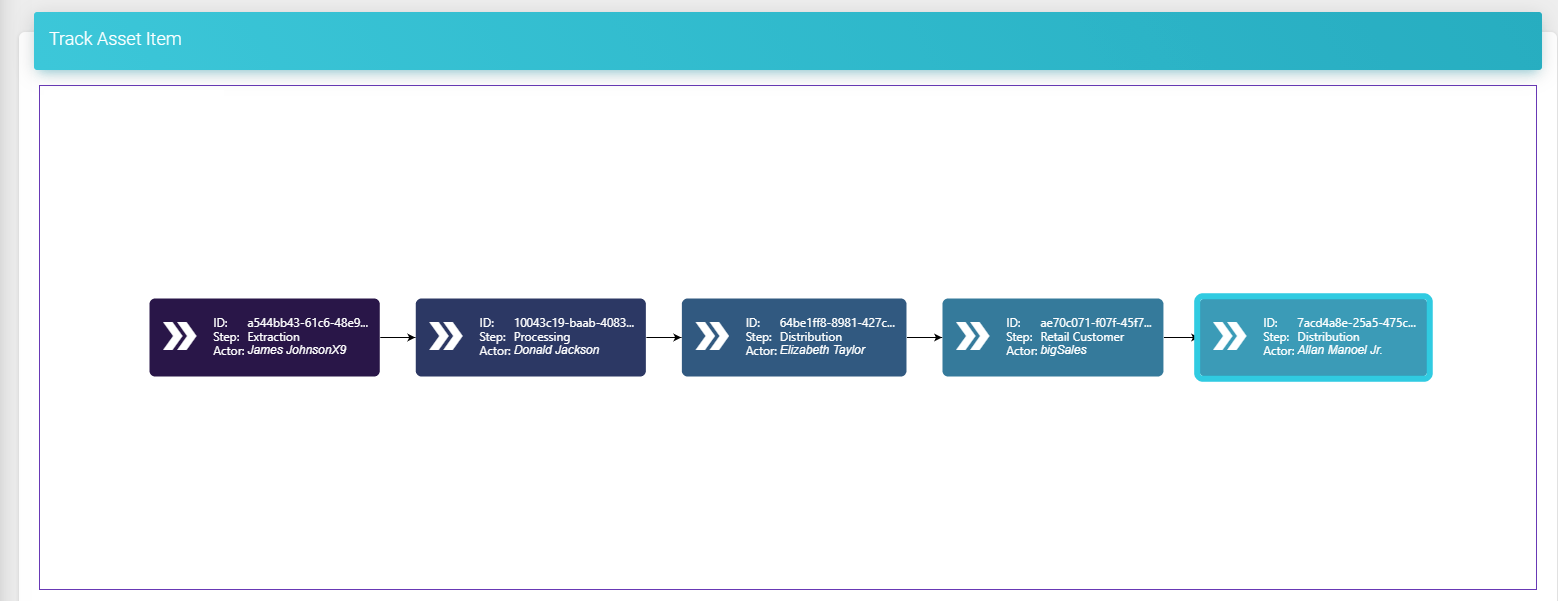
\includegraphics[scale=0.375]{images/use_example/trackbackwards.png}
\caption{Track an asset item backward.}
\label{fig:track_asset_item}
\end{center}
\end{figure}

Usage of blockchain helped to solve the problem since all the information under the blockchain is immutable. It can be audited since the information is stored and cannot be modified or deleted. The system allows anyone to check the previous' records traceability, which can be achieved by arriving at the beginning of the chain. A blockchain does play a key role in traceability, as it ensures the data logged is not tampered with once it has been saved to the blockchain.
 
 
 
 
 